% This is LLNCS.DEM the demonstration file of
% the LaTeX macro package from Springer-Verlag
% for Lecture Notes in Computer Science,
% version 2.2 for LaTeX2e
%
\documentclass{llncs_Ibergrid2013}
%
\usepackage{makeidx}  % allows for indexgeneration
%
%\usepackage[dvips]{graphicx}
%
\usepackage{epsfig}
\usepackage{cite}
\usepackage{url}
\usepackage{microtype}
\usepackage[english]{babel}
\usepackage{graphicx}
\usepackage{eurosym}
\usepackage{url}
\usepackage{multirow}
\usepackage{listings}
\usepackage{natbib}
\begin{document}
%
\frontmatter          % for the preliminaries
%
\pagestyle{headings}  % switches on printing of running heads
\addtocmark{Federated Appliance Distribution in a Federated Cloud} % additional mark in the TOC
%
\mainmatter              % start of the contributions
%
\title{Federated Appliance Distribution in a Federated Cloud}
%
\titlerunning{VM Image Management}  % abbreviated title (for running head)
%                                     also used for the TOC unless
%                                     \toctitle is used
%
\author{A. Sim\'on\inst{1}, E. Freire\inst{1}, R. Rosende\inst{1}, I. D\'iaz\inst{1}, A. Feij\'oo\inst{1}, P. Rey\inst{1}, J. L\'opez-Cacheiro\inst{1}, C. Fern\'andez\inst{1} and O. Synge\inst{2}}
%
%\authorrunning{First Author et al.}   % abbreviated author list (for running head)
%
%%%% modified list of authors for the TOC (add the affiliations)
\tocauthor{First Author (Institution of first author's affiliation),
Second Author (Institution of second author's affiliation)}
%
\institute{Fundaci\'on Centro de Supercomputaci\'on de Galicia, Santiago de Compostela, Spain\\
\email{grid-admin@cesga.es}
\and
\email{owen.synge@jaysnest.de}
}




\maketitle              % typeset the title of the contribution

\begin{abstract}
With the development of Federated cloud infrastructures, Maintainers of virtual appliances need a mechanism to distribute thier work to sites, ideally without external dependancies that may delay critical updates to virtual appliances. This paper summarises the work developed within EGI FedCloud taskforce during the last year to deploy a sustainable federated VM image management using a decentralised approach connecting sites to scientists with minimal overhead.
\end{abstract}

%
\section{Introduction}
\label{sect-introduction}
%
With virtual appliances on Cloud IaaS resources the complications for integrating multiple components and dependencies of a service can be managed closer to the appliance creator and maintainer without need for the cloud provider to be involved. Cloud IaaS has shown great commercial success, so much so that new cloud software stacks are being developed, and many companies and research institutes are deploying these clouds for both internal and external use. EGI-inspire brings together many sites, running multiple IaaS Cloud implementations as a Federated cloud. As part of this effort they are making efforts to help abstract away these differences so that Virtual Appliance users and maintainers can remain IaaS implementation and site neutral.

However Cloud implementation neutrality increases the interoperability challenges. A federated cloud increases this difficulty still further, as different clouds with corresponding APIs, Appliance formats, and different contextualisation mechanism must be supported in a truly federated Cloud. 

Interoperability of Appliance distribution is one of the first dependencies in the process, of creating a federated cloud, This paper is focused on some of the issues surrounding Virtual Appliance Image Management in a federated cloud environment and how it was solved by EGI FedCloud taskforce.

It is organised in the following sections. First, Section~\ref{sect-relatedwork} presents the state of the art regarding cloud frameworks with virtual appliance management, Section~\ref{sect-vmcaster} describes the VMcaster/VMcatcher image management tools, how it was implemented by EGI FedCloud project and how it was configured at CESGA. 
Section~\ref{sect-handlers} explains how VMcatcher event handlers work, and how allow different plugins for cloud frameworks like OpenNebula or OpenStack to synchronize VM images between heterogeneous cloud technologies. 
Finally Section~\ref{sect-conclusions} will present the conclusions and future work.  

%\subsection{User Services}


%\begin{figure}[h!]
%\centering
%\includegraphics[width=60mm,angle=90]{./PSFIGs/user-services.eps}
%\caption{Use case in IBERGRID}\label{figUSER}
%\end{figure}
\section{Related Work}
\label{sect-relatedwork}
The use of Cloud infrastructures in science has been documented, and it is a very promising field, but integrating Clouds with the Grid is a challenge, as related on Dillon et al.~\cite{Dillon2010}. Goasguen et al.~\cite{Goasguen2012} presents the results of an internal production cloud service in CERN and suggestions to expand it to another Grid sites. Zhao et al.~\cite{Zhao2012} presents a infrastructure of a dozen computing sites using OpenNebula as the management solution. It concludes that Clouds are very useful for science, but there are still many performance issues to be resolved. Hoffa et al.~\cite{Hoffa2008} reached similar conclusions regarding cloud vs local deployments.

There are also many works that compare the different solutions for VM Management, like Xiaolong et al.~\cite{Xiaolong2012}, which compares OpenNebula and Openstack, and Laszewski et al.~\cite{Laszewski2012}, which does a more complete survey including Eucalyptus, Nimbus and some other solutions. The existence of numerous trade-offs and fragmented market for these tools motivated us to support cross-grid environments.

On the realm of security, our solution emphasizes the authentication of users and the validation of VMs. There are other works on the area, but some, like Xi et al.~\cite{Xi2012} are concerned more with running trusted VMs on on untrusted environments, which can be seen as the opposite problem, and many others, like Schwarzkopf et al.~\cite{Schwarzkopf2012} are concerned with improving the internal security of VMs maintained by Cloud users instead of infrastructure operators.

There are still other comparable solutions, Lagar-Cavilla et al.~\cite{Lagar-Cavilla2009} use a non-local fork mechanism to spawn many copies of a VM across many sites, but this method would be at odds with current Grid practices. Diaz et al.~\cite{Diaz2012} have a similar system that bridges OpenNebula and OpenStack, but it uses the Amazon EC2 API, which has licensing issues preventing us for using it, and does not address the authorization and validation of VMs. On a more partial resemblance, Maurer et al.~\cite{Maurer2013} also automates some aspects of VM management and updates using an autonomous system, and Django et al.~\cite{Django2013} changes the context of VMs on the fly to do load balancing and improve brokering. This last functionality would be invaluable for Grid operators, which must frequently tend to processes that get stuck due to unrealistic brokering requirements, and would also avoid many downtimes due to reconfiguration.



\section{VMcaster/VMcatcher image management interface}
\label{sect-vmcaster}
VMcaster~\cite{vmcaster} and VMcatcher~\cite{vmcatcher} are two different tools to generate and subscribe to virtual machine image lists.
These tools use an internal database (similar to a podcast syndication or a Linux package manager) where images information and lists are stored into an internal SQLite database.
SQLite has proved more than adequate for the low transaction rate of a image list subscriber and so deployment issues are just backing up a database file.
In many senses VMcaster/VMcatcher tools are similar to Debian's \textit{aptitude} or RedHat's \textit{yum} utilities. 

These tools try to match the requirements set by the now completed HEPiX virtualisation working group~\cite{hepix}.
The main task of this working group was to provide to sites a way to control and mange Virtual Machine (VM) Image's provided by experiments, and execute the VMs in a trusted environment (similar to the current computing environment provided under Grid computing).
During the last year the EGI federated cloud task force has recommended VMcatcher as well for installation at all cloud resource providers in their collaboration and the status of the integration with OpenStack and OpenNebula.

In this case since the software is made with the Grid in mind and to avoid man in the middle security issues, VMcaster/VMcatcher tools are based on the X.509 certificate authentication model.
All the image lists are signed by an authenticated endorser with his/her personal X.509 certificate. 
This means all images are referenced by an Virtual Machine Image List which contains a secure hash (SHA512) signed using X.509 personal certificates (provided by the image list endorser). 
These Virtual Machine Image Lists are published, and interested sites subscribe to the Lists in a catalogue at the site. 

When it is received an instantiation request, the image validity is checked. If the Virtual Machine Image List is valid, the Image is contextualised and then instantiated (see figure \ref{fig:infrastructure}). 
Using this mechanism a virtual image can be checked for validity, all image lists are signed and it provide a version number and expiration date. If the image list does not satisfy these requirements the image is not instantiated and the request is rejected.
Another important feature of VMcaster/VMcatcher is the support of cloud framework agnostic tools, these tools do not depend on the cloud solution used by the sites. Besides it can be integrated with different frameworks using different plugins to use the new images directly from for example, OpenNebula or OpenStack (see section \ref{sect-handlers} for more information).

\begin{figure}[h]
\centering
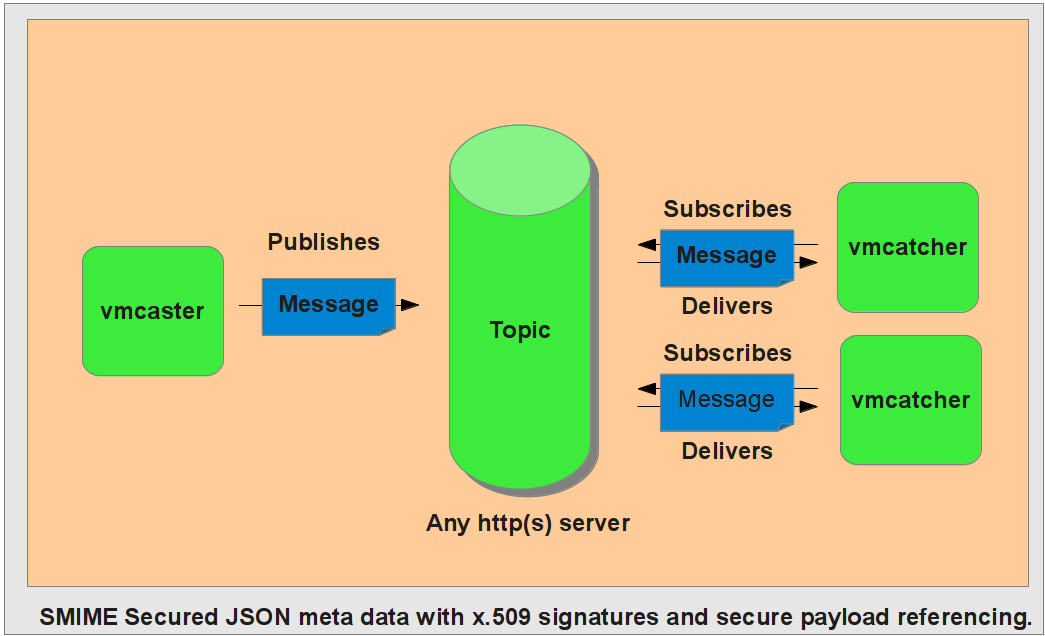
\includegraphics[width=1\textwidth]{vmcaster_vmcatcher.png}
\caption{VMcaster and VMcatcher infrastructure.}
\label{fig:infrastructure}
\end{figure}

\subsection{VMcaster}
VMcaster is a simple tool for publishing, managing and updating virtual machines image lists which follows the HEPix image list specifications.
All the image lists and metadata created by VMcaster are signed and trusted with a X.509 certificate.
This provides a mechanism by which a virtual image can be checked for validity by any subscriber. Any user can check the image list expiration date, if it was revocated or it has been tampered by a third party.
All images and image lists have an UUID. These UUID's should be globally unique and consequently the UUID should be generated using a UUID generator using suitable seeds. As example for Debian, Redhat and Scientific Linux users can execute the following UUID generator:
\begin{verbatim}
$ uuidgen

dfc470ab-0845-4c3b-bc6a-02f990388a17
\end{verbatim}
We can use the new UUID with VMcaster to create a empty image list:
\begin{verbatim}
$ vmcaster --select-imagelist dfc470ab-0845-4c3b-bc6a-02f990388a17 \
--add-imagelist
\end{verbatim}
This command generates an empty image list in our local \textit{vmcaster.db} database (not published yet) with a few predefined objects. We can query the image list ID to see the current object list.
The database information is shown in JSON format:
\begin{verbatim}
$ vmcaster --select-imagelist dfc470ab-0845-4c3b-bc6a-02f990388a17 \
--show-imagelist
{
    "hv:imagelist": {
        "dc:identifier": "dfc470ab-0845-4c3b-bc6a-02f990388a17"
    }
}
\end{verbatim}
The object \textit{dc:identifier} contains always an UUID and it is included in images or image lists. 
At this moment the image list does not include any relevant information but thanks to VMcaster utility the image list endorser can introduce new objects and information.
The most important objects are: the image title, its description, its endpoint (a valid \textit{url}) and also the endorser unique certificate DN. 
These values can be included into the internal database running these commands, as example:
\begin{verbatim}
$ vmcaster --select-imagelist <image_list_UUID> \
--key-set-imagelist "dc:title"\ 
--key-value-imagelist "New Image List"

$ vmcaster --select-imagelist <image_list_UUID> \ 
--key-set-imagelist "dc:source" --key-value-imagelist "CESGA"

$ vmcaster --select-imagelist <image_list_UUID> \ 
--key-set-imagelist "dc:description"\ 
--key-value-imagelist "My image list for internal users"

$ vmcaster --select-imagelist <image_list_UUID> \ 
--key-set-imagelist "hv:uri" --key-value-imagelist \ 
"http://cloud.cesga.es/files/image.list"

$ vmcaster --select-endorser "/DC=es/DC=irisgrid/O=cesga/CN=alvarosimon" \
--key-set-endorser "dc:creator" --key-value-endorser "Alvaro Simon"
\end{verbatim}

Endorsers can also import image lists (in JSON or MIME format) to streamline the image list creation. At this moment the endorser can include new images metadata into the new image list catalogue.
Image insertion procedure is similar to image list creation \textit{vmcaster --select-image <UUID> --key-set-image <IMAGE TAG> --key-value-image <VALUE>}.  
The image list endorser only has to generate a new UUID and insert the relevant objects, in this case:
\begin{itemize}
 \item \textit{dc:title}: Image title name
 \item \textit{sl:comments}: It includes image comments (user login and password, software included etc).
 \item \textit{sl:osversion}: The Operating System version as LSB compliant. As example Scientific Linux release 6.4 (Carbon).
 \item \textit{sl:arch}: System architecture (x86\_64, i386 etc).
 \item \textit{sl:os}: Operating System name (Ubuntu, Debian, RedHat..).
 \item \textit{hv:uri}: Image location endpoint. The image must be accesible from this url. As example \url{http://cloud.cesga.es/images/debian-6.0.5-x86_64-base.qcow2}
 \item \textit{hv:format}: VM image format (QCOW2, RAW)
\end{itemize}
All the new images should be assigned to a image list, we can include the same image in different image lists. To add a new image to a specific image list:

\begin{verbatim}
$ vmcaster --select-imagelist <IMAGE_LIST_UUID> --imagelist-add-image\ 
--select-image <IMAGE_UUID>
\end{verbatim}

VMcaster can be configured to syncronize and upload local images to a specific server endpoint. This mechanism allows to VMcaster users to upload images and image lists to a web server in an automated way.
This information is located into a configuration file (\textit{/etc/vmcaster/vmcaster.cfg}). This mechanism is very useful for Image List endorsers as they can use this configuration file to include several servers to keep the image lists up to date in a short period of time.
\textit{vmcaster.cfg} file uses this schema:
\begin{verbatim}
[SERVER NAME]
server = "myserver.org"
protocol = "scp"
uriMatch = "https://myserver.org/"
uriReplace = "user@myserver.org:/var/www/html/"
\end{verbatim}
In this case VMcaster will use \url{myserver.org} web page to upload any image or image list. 
\textit{vmcaster.cfg} accepts different communication protocols such scp, GSIdCap~\cite{dcache} or a local transmission. If this configuration file is set, VMcaster will upload images automatically using this command:

\begin{verbatim}
vmcaster --upload-image <local_image_path> --select-image <IMAGE_UUID>
\end{verbatim}

VMcaster detects the image size and generates a SHA512 hash for each uploaded image, when this process is complete the updated information is included into the VMcaster database automatically.

At the end the information can be gathered from the local database, as example using JSON format image list:
\begin{verbatim}
{
    "hv:imagelist": {
        "dc:date:created": "2013-03-18T16:52:55Z", 
        "dc:date:expires": "2014-04-15T16:52:55Z", 
        "dc:description": "CESGA image list for internal usage", 
        "dc:identifier": "2204eed5-f37e-45b9-82c6-85697356109c", 
        "dc:source": "CESGA", 
        "dc:title": "CESGA image list", 
        "hv:endorser": {
            "hv:x509": {
                "dc:creator": "Alvaro Simon Garcia", 
                "hv:ca": "/DC=es/DC=irisgrid/CN=IRISGridCA", 
                "hv:dn": "/DC=es/DC=irisgrid/O=cesga/CN=alvarosimon", 
                "hv:email": "asimon@cesga.es"
            }
        }, 
        "hv:images": [
            {
            {
                "hv:image": {
                    "dc:description": "UI-UMD3.0.0", 
                    "dc:identifier":\ 
"9d6b140f-7a08-4f8c-8c25-3564bcb50e33", 
                    "dc:title": "EMI-UI", 
                    "hv:format": "QCOW2", 
                    "hv:hypervisor": "QEMU,KVM",  
                    "hv:uri":\ 
"http://cloud.cesga.es/images/test_ui_image.QCOW2", 
                    "hv:version": "0.0.1", 
                }
            }
        ], 
        "hv:uri": "http://cloud.cesga.es/files/image.list", 
        "hv:version": "2.9"
    }
}
\end{verbatim}
Reading the image list example in JSON format a future subscriber can indentify the available images and also the image list creation/expiration dates or the endorser DN.

When the image list is ready and updated the endorser can publish it to all sites included into \textit{vmcaster.cfg} file. 
The procedure is quite similar to image uploading, but the image must be signed by the endorser certificate to validate its authenticity.
VMcaster asks for user certificate password and upload the image list to its final endpoint, this can be executed with a single command:
\begin{verbatim}
$ vmcaster --select-imagelist <IMAGE_LIST_UUID> --upload-imagelist
\end{verbatim}
This procedure allows different image endorsers to distribute and update image catalogs among different endpoints and sites (which is suitable for a federated architecture).
Besides all image lists has endorsed information about endorser certificate public key, image download endpoint, initial global validity, etc. 
That means valid images can be selected, downloaded and instantiated and tested by different resource provides. 
This task is done by VMcatcher utility described in the next section.


\subsection{VMcatcher}
VMcatcher utility allows image consumers to subscribe to VM Image Lists generated by VMcaster. 
Using this utility users can select and download trusted images.
This utility cache the images selected in a image list, validates the list with X.509 based public key cryptography, and also checks  the images SHA512 hashes. 
Another important feature of VMcaster is that provides events for further applications to process, update or expire changes of virtual machine images. 
These events can be used by event listeners or event handlers to react to specific changes (when a image is set as invalid or a it is available a new image update). 

VMcatcher and VMcaster works in a similar way. The software is based upon a local database that stores subscriptions to VM image lists, registered endorsers, and which images belong to which subscriptions. 
It allows to select images to be selected for subscription. An user can select the desired image lists and then set the desired images subscription.
Subscribed images can be downloaded, verified and cached. VMcatcher also verifies if the cached images have expired or not, and if images are valid or has expired, in which case it is moved to an expiry directory.
The image consumer must trust in a endorser, in this case users can include and trust in a image endorser including his/her X.509 certificate Distinguished Name (DN).
To include a new trusted endorser:
\begin{verbatim}
$ vmcatcher_endorser --create --endorser_uuid='Alvaro Simon' \
--subject='/DC=es/DC=irisgrid/O=cesga/CN=alvarosimon' \
--issuer='/DC=es/DC=irisgrid/CN=IRISGridCA'
\end{verbatim}
And now the user only has to download the desired image list from the endpoint and import it into a local VMcaster database:
\begin{verbatim}
$ wget http://cloud.cesga.es/files/image.list
$ vmcatcher_subscribe -s file:////`pwd`/image.list
\end{verbatim}
At this point the image user can show and select any image UUID from the new list to be downloaded. 
The Image list may vary (image endorse includes new images, revoke old ones, etc), in any case the local image list database should be updated frequently executing the command \textit{vmcatcher\_subscribe -U}.
This command checks the image lists endoint and updates the local database accordingly.
After image selection the images can be downloaded and updated to a local cache running:
\begin{verbatim}
$ vmcatcher_cache
\end{verbatim}

The new downloaded images are stored into \textit{<VMCATCHER\_DIR>/cache} directory, meanwhile revoked or expired images are moved to \textit{<VMCATCHER\_DIR>/cache/expired} directory. 
This mechanism prevents that old or revoked images are used by mistake. VMcatcher also raises some events if the image is downloaded, revoked or removed. 
These pre-defined events can be used by the cloud frameworks to perform different actions.

\section{Image management event handlers}
\label{sect-handlers}
VMcatcher and VMcaster are useful tools to disseminate and keep updated our images but they do not interact with cloud frameworks directly.
VMcatcher was written in Python and generates pre-defined events that can be received by an asynchronous callback subroutine or event handler.
Fortunately the cloud community has developed event handlers to interact with the most popular frameworks like OpenNebula or CloudStack.
OpenNebula event handler~\cite{onevent} was developed by the CESGA team and currently is available from the VMcaster repository. 
The \textit{vmcatcher\_eventHndlExpl\_ON} package provides a new python and cron script which detects VMcatcher events. 
This script detects several VMcatcher event types. In this case OpenNebula handler only waits for a new Expire or Available VMcatcher event.
If VMcatcher raises a \textit{AvailablePostfix} event, this is detected by \textit{vmcatcher\_eventHndlExpl\_ON} event handler and reads the new image attributes such UUID, image name, description and image format.
\begin{figure}[h]
\centering
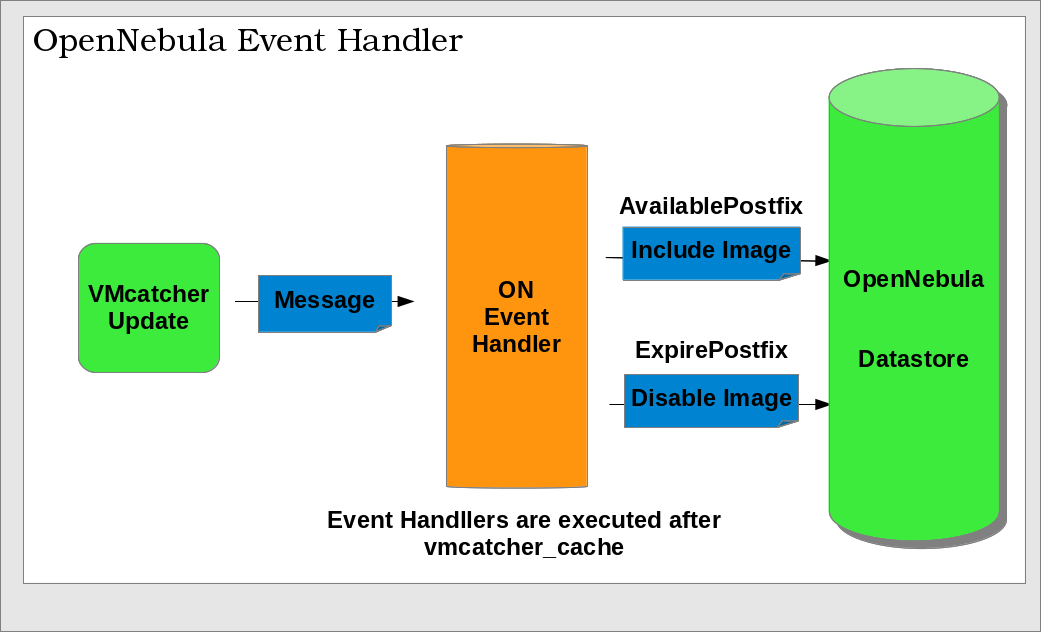
\includegraphics[width=1\textwidth]{ONeventhandler.png}
\caption{OpenNebula event handler.}
\label{fig:onevent}
\end{figure}
If a new image is downloaded (\textit{AvailablePostfix} event), the OpenNebula event handler gets the image information, generates a new OpenNebula template and includes the new image into the local OpenNebula datastore (see figure \ref{fig:onevent}). 
For security reasons, the new images are not public, they are only available for the oneadmin user. The OpenNebula administrator should verify the new image first (checking its contextualisation script, if the image is executed correctly etc).
After this period of time the image status is changed to be available for external users. 
Moreover if VMcatcher detects an image revocation the OpenNebula event handler search the image UUID from OpenNebula image database and it is set to disable status.
The image is not removed by the event handler, it should be removed by the site administrator from the OpenNebula datastore.

The OpenNebula event handler is not the only one. OpenStack administrators can also use Glancepush~\cite{glancepush} service to keep their local image catalog updated. 
This service was developed at IN2P3 and it works in a similar way than the OpenNebula event handler. 
In this case Glancepush updates the OpenStack Image Service (Glance) if it detects any image change from VMcatcher tool. 
The new package (\textit{glancepush-vmcatcher}) is available from IN2P3 ftp server, and it only requires a working glance service and an OpenStack user account to push images into the catalog.

%\section{Use Case: EGI SA2.3 verification image repository}
%\label{sect-usecase}
%This is my text 

\section{Conclusions and Future work}
\label{sect-conclusions}
The management of virtual machine images is a critical task within a federated cloud architecture. It involves certain safety standards and special scalability and availability and stability patterns.
Taking these requirements into account Fedcloud taks force have chosen VMcaster and VMcatcher utilities to distribute and validate VM images between the resource providers.
Fedcloud resource providers are using a heterogenous cloud frameworks ecosystem (OpenStack, OpenNebula, WNoDES~\cite{wnodes}, etc). This kind of federated infrastructure requires agnostic tools.
Fortunately as we have explained in this paper, VMcatcher can be used by any cloud framework to distribute and update images in a transparent way. 
The new image management tools are being used by EGI Fedcloud providers since last year successfully and probably it will be used in more use cases in the near future.

A new use cases is the EGI SA2.3 verification image repository. The EGI SA2 testbed is used to verify and test the new middleware before reaching the production software repository (UMD).
One of the most important new features is the ability to distribute and publish VM images in an automated way. 
These new tools, like EGI MarketPlace\footnote{EGI MarketPlace: \url{http://marketplace.egi.eu}} and VMcatcher\footnote{VMcatcher: \url{https://github.com/hepix-virtualisation/vmcatcher}} can be also used within SA2 verification process to distribute and publish new UMD services after its verification. 
This work is still on going and it will be available in the next months. Using this infrastructure the new EGI certified image it will be available to be used and tested by EGI site administrators after each successful verification.
For the moment after each software verification the images are stored locally into CESGA OpenNebula datastore but thanks to image management tools like VMcaster the new images will be published in an automated way.
This new paradigm will be useful to users that want to check the latest software changes without the need to install a new service from scratch.


\section*{Acknowledgements}
\label{sect-acknowledgements}
This work is partially funded by the  EGI-InSPIRE (European Grid Initiative: Integrated Sustainable
Pan-European Infrastructure for Researchers in Europe) is a project co-funded by the European Commission 
(contract number INFSO-RI-261323) as an Integrated Infrastructure Initiative within the 7th Framework 
Programme. EGI-InSPIRE began in May 2010 and will run for 4 years. Full information is available at:
\url{http://www.egi.eu/}.

%
% ---- Bibliography ----
%
%\begin{thebibliography}{99}
%
\bibliographystyle{abbrv}

%\bibliographystyle{thebibliography}
\bibliography{bibliography}

%\bibitem{dcache}
%\newblock The dcache book. 
%\newblock \url{http://www.dcache.org/manuals/Book/}, May 2013.

%\bibitem{Django2013}
%\newblock D. Armstrong et al.
%\newblock Runtime virtual machine recontextualization for clouds.
%\newblock Euro-Par 2012: Parallel Processing Workshops. Volume 7640 of Lecture Notes in Computer Science, pages 567--576. Springer Berlin Heidelberg, 2013.

%\bibitem{hepix}
%T.~Cass.
%\newblock The hepix virtualisation working group: Towards a grid of clouds.
%\newblock {\em Journal of Physics: Conference Series}, 396(3):032020, 2012.

%\bibitem{Diaz2012}
%J.~Diaz, G.~von Laszewski, F.~Wang, and G.~Fox.
%\newblock Abstract image management and universal image registration for
%  {C}loud and {HPC} infrastructures.
%\newblock In {\em Cloud Computing (CLOUD), 2012 IEEE 5th International
%  Conference on}, pages 463--470, 2012.

%\bibitem{Dillon2010}
%T.~Dillon, C.~Wu, and E.~Chang.
%\newblock Cloud computing: Issues and challenges.
%\newblock In {\em Advanced Information Networking and Applications (AINA), 2010
%  24th IEEE International Conference on}, pages 27--33, 2010.

%\bibitem{Lagar-Cavilla2009}
%L.-C. et~al.
%\newblock Snowflock: rapid virtual machine cloning for cloud computing.
%\newblock In {\em Proceedings of the 4th ACM European conference on Computer
%  systems}, EuroSys '09, pages 1--12, New York, NY, USA, 2009. ACM.

%\bibitem{Goasguen2012}
%S.~Goasguen, B.~Moreira, E.~Roche, and U.~Schwickerath.
%\newblock Lxcloud : a prototype for an internal cloud in hep. experiences and
%  lessons learned.
%\newblock {\em Journal of Physics: Conference Series}, 396(3):032098, 2012.

%\bibitem{Hoffa2008}
%C.~Hoffa, G.~Mehta, T.~Freeman, E.~Deelman, K.~Keahey, B.~Berriman, and
%  J.~Good.
%\newblock On the use of cloud computing for scientific workflows.
%\newblock In {\em eScience, 2008. eScience '08. IEEE Fourth International
% Conference on}, pages 640--645, 2008.

%\bibitem{Xi2012}
%C.~Li, A.~Raghunathan, and N.~Jha.
%\newblock A trusted virtual machine in an untrusted management environment.
%\newblock {\em Services Computing, IEEE Transactions on}, 5(4):472--483, 2012.

%\bibitem{Maurer2013}
%M.~Maurer, I.~Brandic, and R.~Sakellariou.
%\newblock Adaptive resource configuration for cloud infrastructure management.
%\newblock {\em Future Generation Computer Systems}, 29(2):472 -- 487, 2013.

%\bibitem{glancepush}
%M.~Puel.
%\newblock Openstack glancepush service.
%  \url{https://github.com/EGI-FCTF/glancepush/wiki}, 2013.

%\bibitem{onevent}
%R.~Rosende.
%\newblock Opennebula event handler.
%  \url{https://github.com/grid-admin/vmcatcher\_eventHndlExpl\_ON}, May 2013.

%\bibitem{wnodes}
%D.~Salomoni, A.~Italiano, and E.~Ronchieri.
%\newblock Wnodes, a tool for integrated grid and cloud access and computing
%  farm virtualization.
%\newblock {\em Journal of Physics: Conference Series}, 331:052017, 2011.

%\bibitem{Schwarzkopf2012}
%R.~Schwarzkopf, M.~Schmidt, C.~Strack, S.~Martin, and B.~Freisleben.
%\newblock Increasing virtual machine security in cloud environments.
%\newblock {\em Journal of Cloud Computing}, 1(1):1--12, 2012.

%\bibitem{vmcaster}
%O.~Synge.
%\newblock Vmcaster vm image publication tool.
%  \url{https://github.com/hepix-virtualisation/vmcaster}, May 2013.

%\bibitem{vmcatcher}
%O.~Synge.
%\newblock Vmcatcher image subscription tool.
%  \url{https://github.com/hepix-virtualisation/vmcatcher}, May 2013.

%\bibitem{Laszewski2012}
%G.~von Laszewski, J.~Diaz, F.~Wang, and G.~Fox.
%\newblock Comparison of multiple cloud frameworks.
%\newblock In {\em Cloud Computing (CLOUD), 2012 IEEE 5th International
%  Conference on}, pages 734--741, 2012.

%\bibitem{Xiaolong2012}
%X.~Wen, G.~Gu, Q.~Li, Y.~Gao, and X.~Zhang.
%\newblock Comparison of open-source cloud management platforms: Openstack and opennebula.
%\newblock In Fuzzy Systems and Knowledge Discovery (FSKD), 2012 9th
%\newblock  International Conference on, pages 2457--2461, 2012.

%\bibitem{Zhao2012}
%Y.~Zhao, Y.~Zhang, W.~Tian, R.~Xue, and C.~Lin.
%\newblock Designing and deploying a scientific computing cloud platform.
%\newblock In {\em Grid Computing (GRID), 2012 ACM/IEEE 13th International
%  Conference on}, pages 104--113, 2012.

%\end{thebibliography}


\end{document}
